\begin{intro}
\label{intro}

En la naturaleza, es posible encontrar de forma ubicua, estructuras alargadas (filamentos), las que conforman redes entre sí. La conformación de estas estructuras complejas y din\'amicas se puede observar en ejemplos particulares como en una red de prote\'inas de una c\'elula eucariota, as\'i como en bacterias, ya que a pesar que pertenecer a distintas familias, ambas tienen estructuras formada por filamentos. 
Caracter\'isticas f\'isicas de estas redes generan propiedades tales como la presencia o ausencia de ciclos, o la posibilidad de dividir o no cada filamento. Por su parte, el análisis de filamentos que conforman la red, puede indicar el estado de \'esta, respecto a su ambiente o de su interior, as\'i como develar informaci\'on relevante sobre la relaci\'on entre la estructura biol\'ogica y funciones fisiol\'ogicas.  
%movimiento interno, reparación de tejido,
% estructuras dinamicas y complejas que juegan varios roles
% A modo de ejemplo, una red de proteinas de una c\'elula eucariota contiene tres tipos de filamentos en la constituci\'on de su citoesqueleto: microfilamentos, microt\'ubulos y filamentos intermedios. Sin embargo, una estructura de citoesqueleto también existe en una bacteria.
  
%\vspace{.5cm}
Los m\'etodos actuales para analizar las redes mencionadas se basan en el procesamiento directo de im\'agenes obtenidas a partir de microscop\'ia (Figura \ref{Fig1a}), pasando por etapas de segmentaci\'on (Figura \ref{Fig1b}), para luego utilizar diversas t\'ecnicas como esqueletonizaci\'on (Figura \ref{Fig1c}), la transformada de Rad\'on o {\it template matching}. Esto permite identificar el grafo que representa a la red (Figura \ref{Fig1d}) o sirve de base para el uso de heur\'isticas que permiten identificar los filamentos de forma individual.
 %como tambi\'en pueden utilizarse una esqueletonizaci\'on de la misma (Figura \ref{Fig1c}), o la construcci\'on de un grafo (Figura \ref{Fig1d}), entre otras.
 % En todos estos casos, el objetivo radica en
La individualizaci\'on de filamentos permite cuantificar las propiedades de la red tales como n\'umero de filamentos, largo de estos, volumen, o curvatura. Estos m\'etodos, basados en la observaci\'on mediante microscop\'ia \'optica tienen como cota m\'axima de resoluci\'on el l\'imite de difracci\'on, $\lambda/2$. Donde $\lambda$ es la longitud de onda de la luz utilizada (o color). Este l\'imite establece que 2 objetos cuya distancia sea inferior a $\lambda/2$ no pueden ser diferenciados, conllevando a que dos partes del grafo cercanos puedan ser observadas como una, dificultando su estudio. Lo anterior es relevante para asociar las propiedades de la red a los v\'ertices del grafo extra\'ido, dando pie a la caracterizaci\'on del mismo (Figura \ref{Fig2a}).
 % vertices del grafo extraido, que representan a un filamento de forma individual, 
 
 \begin{figure*}[h!]
    \centering
    \label{fig:flujo-expected}
    \begin{subfigure}[t]{0.5\textwidth}
        \centering
        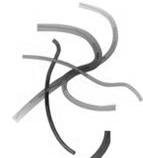
\includegraphics[height=1.5in]{imagenes/define-weighted-4.png}
        \caption{Representaci\'on simplificada de una red con cruces y sobreposici\'on de filamentos en una imagen de microscop\'ia.}
        \label{Fig1a}
    \end{subfigure}%
    ~ 
    \begin{subfigure}[t]{0.5\textwidth}
        \centering
        
\includegraphics[height=1.5in]{imagenes/define-weighted-4-bw-invert.png}
        \caption{Preprocesamiento de la imagen mediante segmentaci\'on para la extracci\'on de la red.}
        \label{Fig1b}
    \end{subfigure}
    %\caption{Caption place holder}
%\end{figure*}
\vskip\baselineskip
%\begin{figure*}[t!]
%    \centering
    \begin{subfigure}[t]{0.5\textwidth}
        \centering
        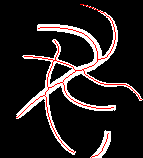
\includegraphics[height=1.5in]{imagenes/skel_in_segment.png}
	    \caption{Esqueletonizaci\'on representativa de la red sobre la imagen de \ref{Fig1b}.}
        \label{Fig1c}
    \end{subfigure}%
    ~ 
    \begin{subfigure}[t]{0.5\textwidth}
        \centering
        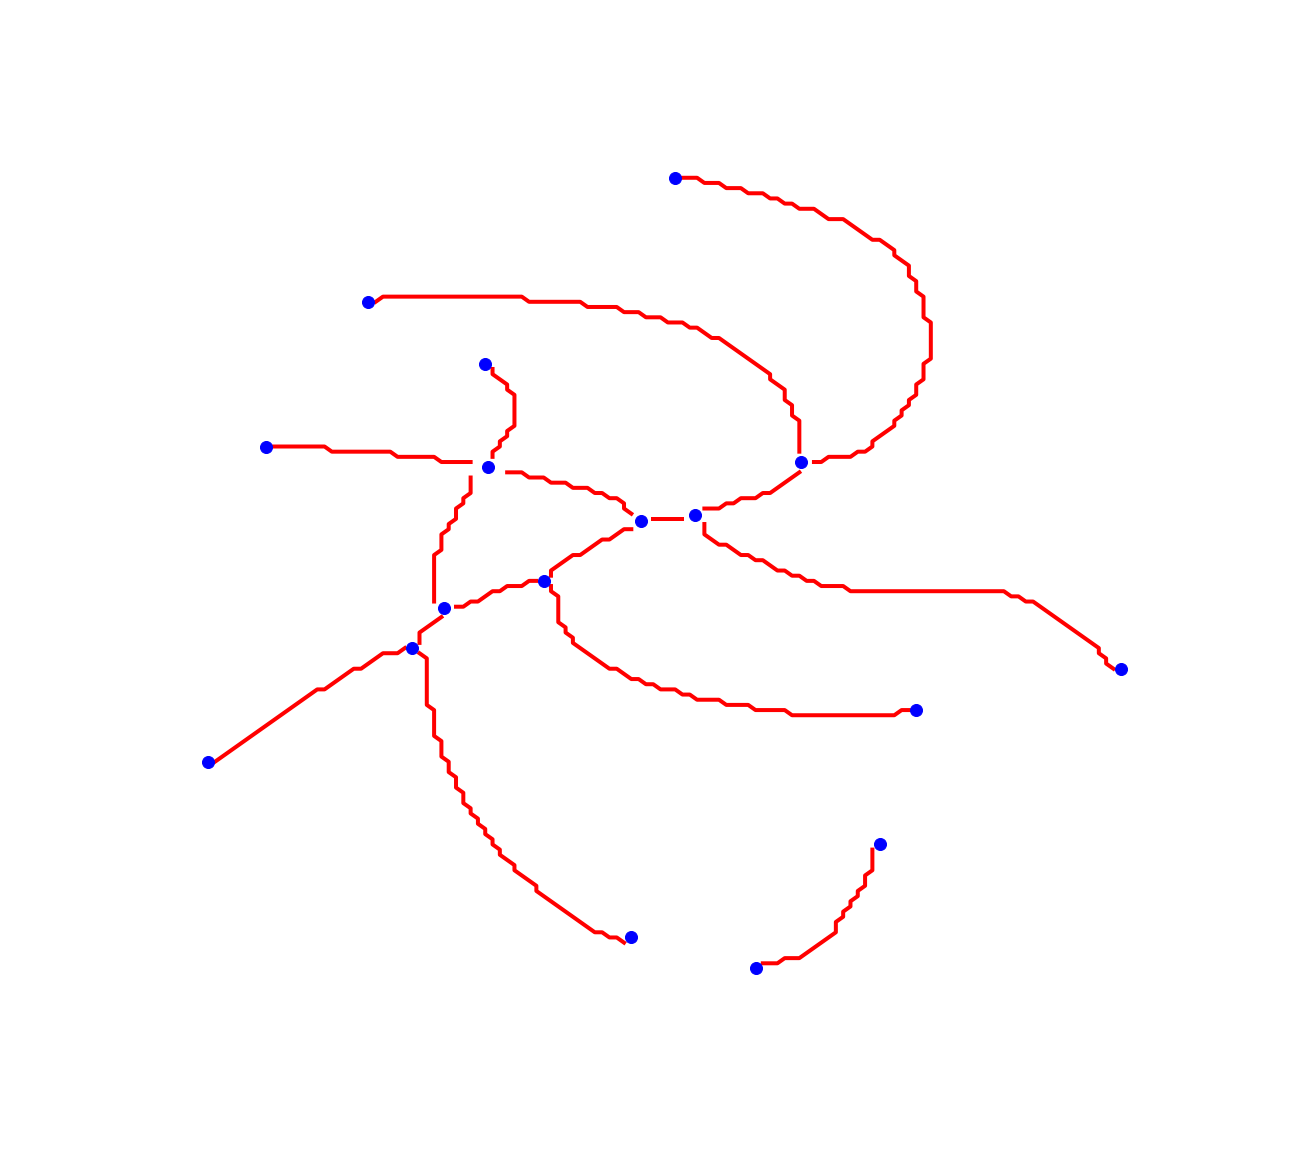
\includegraphics[height=1.5in]{imagenes/graph_of_skel_no_axis.png}
        \caption{Grafo que representa la esqueletonizaci\'on de la red.}
        \label{Fig1d}
    \end{subfigure}
%    \vskip\baselineskip
    \caption{Procedimiento para obtener un grafo que representa la red, a partir del procesamiento de una imagen de microscop\'ia, utilizando segmentaci\'on y esqueletonizaci\'on. Fuente: \cite{breuer2015define}}
\end{figure*}

Existen investigaciones en la literatura que apuntan a las distintas etapas de este problema, las que tienen en com\'un el uso de t\'ecnicas del \'area de procesamiento de im\'agenes para el tratamiento inicial de la imagen de microscop\'ia. La individualizaci\'on de filamentos puede ser categorizado en: basado en procesamiento de im\'agenes o como un problema de optimizaci\'on. 
En ambas categor\'ias, las cr\'iticas m\'as repetidas en los trabajos del \'area suelen ser la cantidad de par\'ametros y la dificultad en su ajuste, en las diversas herramientas existentes. Un segundo problema com\'un es que la obtenci\'on de informaci\'on relacionada a la morfolog\'ia y el comportamiento de las redes es m\'as cualitativo que cuantitativo \cite{asgharzadeh2018computational}\cite{qiu2014quantitative}, lo que supone un problema al trasladar el  an\'alisis a una gran cantidad de datos, dado que cada enfoque es demasiado espec\'ifico a su correspondiente software.

\begin{figure*}[h]
    \begin{subfigure}[t]{0.5\textwidth}
        \centering
        
\includegraphics[height=1.2in]{imagenes/define-weighted-4-expected2.png}
        \caption{Visualizaci\'on de un resultado posible de individualizaci\'on, limitando los filamentos identificados a estructuras simples.}
        \label{Fig2a}
    \end{subfigure}
    ~ 
    \begin{subfigure}[t]{0.5\textwidth}
        \centering
        
\includegraphics[height=1.2in]{imagenes/define-weighted-4-expected1.png}
        \caption{Visualizaci\'on de otro resultado posible de individualizaci\'on, permitiendo filamentos m\'as complejos.}
        \label{Fig2b}
    \end{subfigure}
	\caption{Posibles resultados de la identificaci\'on de filamentos. El resultado esperado de esta investigaci\'on es asociar a cada arista del grafo, como el de la figura \ref{Fig1d}, un peso que pondere diversos criterios como \'angulo de bifurcaci\'on del filamento, grosor y/o largo. Al plantearlo como un problema de optimizaci\'on, la ponderaci\'on y otras restricciones, entregar\'an resultados como la imagen \ref{Fig2a} o \ref{Fig2b}, expresado gr\'aficamente mediante gradiente de colores. Fuente: Elaboraci\'on propia}
\end{figure*}

En resumen, el problema de identificar filamentos en im\'agenes de microscop\'ia esta limitado por la resoluci\'on, y los problemas de m\'ultiples par\'ametros a ajustar, para los m\'etodos basados en procesamiento de im\'agenes, el costo computacional en los m\'etodos basados en optimizaci\'on, y falta de descriptores cuantitativos en ambas. La revisi\'on bibliogr\'afica da cuenta tambi\'en de pocas herramientas disponibles. Todo lo anterior implica que parte del an\'alisis deba ser manual, lo que para grandes cantidades de datos, hace los estudios m\'as propensos a errores. 

\section*{Hip\'otesis y Objetivos}
Como se ha presentado, los m\'etodos de individualizaci\'on de filamentos que s\'olo usan herramientas de procesamiento de im\'agenes, pueden representar la red a trav\'es de los filamentos que la conforman, sin embargo para realizar mediciones cuantitativas requieren ajustar m\'ultiples par\'ametros. Por otra parte los m\'etodos de optimizaci\'on permiten reducir los par\'ametros, pero con un alto costo computacional, el que puede ser abordado con el uso de heur\'isticas o algoritmos de aproximaci\'on. Tambi\'en se debe tener en consideraci\'on en ambos m\'etodos, el n\'umero de caracter\'istica utilizadas al momento de realizar la individualizaci\'on. Esto nos permite establecer la pregunta:

\smallskip
¿Es posible determinar correctamente la cantidad de filamentos, desarrollando un modelo de optimizaci\'on que utilice una combinaci\'on de m\'ultiples caracter\'isticas como el largo, grosor, \'angulo de bifurcaci\'on, curvatura o direcci\'on, tanto en la asignaci\'on de pesos como en la selecci\'on del subconjunto de caminos?
\smallskip

% costo computacional de m\'etodos de optimizaci\'on es abordado con algoritmos de aproximación o heurísticas
% Solucion actual propuesta en Define aborda el recorrido de grafos considerando como peso solo 1 valor que representa una caracteristica de la arista, 
% pregunta es si se puede determinar la cantidad de filamentos utilizando un peso que agrupe/pondere varias caracteristicas
%(geometricos comunmente)
% Entre las investigaciones y herramientas existentes derivadas de los mismos, 
%- overlap, intensidad, fragmentación

Dado que en el problema de individualizaci\'on de filamentos se desconoce el origen y fin de cada filamento al iniciar la resoluci\'on del problema, plantear un recorrido de grafos puede resultar computacionalmente costoso, lo que puede ser evitado al plantear un modelo de optimizaci\'on que pueda hacer la asociaci\'on entre aristas que sean parte del mismo filamento.

Se debe agregar que existe informaci\'on \textit{a priori}, indicada por el tipo de estructura observada, la cual restringe los comportamientos posibles de la red. Por ejemplo, los filamentos de prote\'ina actina no se pegan entre s\'i, formando estructuras sin ciclos, mientras que el ret\'iculo endoplasm\'atico (organelo celular encargado principalmente de la s\'intesis de prote\'inas) si presenta ciclos. Estas condiciones pueden aportar limites m\'as acotados a algunos de los criterios de cuantificaci\'on y es conocimiento disponible previo a la observaci\'on en el microscopio. Es importante destacar que alguna de la informaci\'on {\it a priori} corresponde a reglas emp\'iricas, que tambi\'en deben ser consideradas durante el an\'alisis.

En base a lo anterior, la hip\'otesis de esta investigaci\'on se basa en que a partir de un grafo con pesos, no dirigido, con o sin ciclos, que representa una red de filamentos, en conjunto con utilizar una combinaci\'on de caracter\'isticas de los segmentos de filamentos como largo, grosor, \'angulo de bifurcaci\'on o curvatura, sumado a la incorporaci\'on de informaci\'on previa disponible sobre el tipo de c\'elula (red de filamentos con o sin ciclos), es posible identificar a cada filamento en la red resolviendo un modelo de optimizaci\'on.

Para validar esta hip\'otesis, se propone realizar los siguientes objetivos:
\subsection*{Objetivo General}
Desarrollar un modelo de optimizaci\'on para la individualizaci\'on de filamentos a partir de un grafo representativo de la red de filamentos, evaluando la variaci\'on en el resultado con distintas combinaciones entre las propiedades de cada segmento de filamento como el grosor, largo, \'angulo de bifurcaci\'on o direcci\'on.
%y que incorpore la informaci\'on {\it a priori} disponible

\subsection*{Objetivos Espec\'ificos}
\begin{itemize}
    \item Generar un modelo de optimizaci\'on para la identificaci\'on de filamentos a partir de un grafo con pesos que representa la red de filamentos.
    \item Implementar un algoritmo que resuelva el modelo de optimizaci\'on, entregando como salida la identificaci\'on de filamentos, considerando casos de solapamiento y/o cruce.
    \item Identificar la ponderaci\'on de propiedades que entregue mejores resultados para grafos que representen una neurona, una bacteria y una c\'elula eucariota de planta.
    \item Evaluar t\'ecnicas que usan s\'olo herramientas de visi\'on por computador, como \cite{boudaoud2014fibriltool}, basada en poblaci\'on de p\'ixeles y \cite{xu2015soax}, que utiliza un m\'etodo derivado de contornos activos. 
    
    %una soluci\'on exacta o aproximada respecto a la individualizaci\'on, dependiendo de la complejidad computacional del problema. 
\end{itemize}

%\subsubsection{Contribuci\'on}

% Contribuci\'on:
Como resultado de los objetivos planteados, se obtendr\'a una herramienta para el an\'alisis automatizado de estructuras de filamentos, lo que permitir\'ia mejorar el seguimiento de procesos din\'amicos o la identificaci\'on de procesos patol\'ogicos de forma autom\'atica.

\section*{Estructura de esta tesis}
lorem lorem ipsum

%\begin{teo}
%Se tiene que $$\int_0^t e^sds=e^t-1.$$
%\end{teo}
\end{intro}